% Chapter Template

\chapter{Analytical Solution} % Main chapter title

\label{Chapter1}

\lhead{Chapter 1. \emph{Analytical Solution using Fourier Series}} % Change X to a consecutive number; this is for the header on each page - perhaps a shortened title

%----------------------------------------------------------------------------------------
%	SECTION 1
%----------------------------------------------------------------------------------------

\section{Coefficients of complex exponential Fourier series :} 
We know that we can express a periodic function f(t) as the following 
\begin{align*}
&f(t) = \sum\limits_{n=-\infty}^{n=\infty} C_n e^{j n\omega t} \\
&f(t) = .....+C_{-1}e^{-j\omega t} + C_0 + C_1e^{j\omega t}+.....
\end{align*}
where
\begin{itemize}
\item \textbf{Constant Term :} 
\begin{align*}
&\boxed{C_0 = \frac{1}{T}\int\limits_0^T f(t) dt}
\end{align*}
\item \textbf{$C_k$ term :} 
\begin{align*}
&\boxed{C_k = \frac{1}{T}\int\limits_0^Tf(t)e^{-j\omega kt}dt}
\end{align*}
\end{itemize}
\section{Applying this to given question :} 

In the question we are given with a input signal defined as \\
V(t) = $\begin{cases}
A & 0\leq t \leq \alpha T \\
0 & \alpha T \leq t \leq T
\end{cases}$ \\
Here A = 10 , but we are making it to generalize for any value. \\
The differential equation we get is 
\begin{align*}
L\frac{di}{dt} + iR =V(t)
\end{align*}
The idea we use here is , We write the V(t) in the RHS as sum of complex exponentials and solve the differential equation for individual complex exponential function and add up all the solutions we get to get the current i(t) (Using superposition principle).\\
Let 
\begin{align*}
V(t) = \sum\limits_{n=-\infty}^{n=\infty} C_n e^{j n\omega t}
\end{align*}
Where $\omega = \frac{2\pi}{T}$ \\
Now let us find the coefficients.
\begin{itemize}
\item \textbf{Constant term :} 
\begin{align*}
C_0 &= \frac{1}{T}\int\limits_0^T V(t) dt \\ 
& = \frac{1}{T} \int\limits_0^{\alpha T}A dt + \int\limits_{\alpha T}^T0dt \\
& = \frac{1}{T} [At]_0^{\alpha T} + 0 \\
& = \frac{1}{T} (A \alpha T ) \\
& = A \alpha \\
&\boxed{C_0 = A\alpha}
\end{align*}
\item \textbf{$C_1,C_2,...,C_k$ terms :} 
\begin{align*}
C_k &= \frac{1}{T}\int\limits_0^Tf(t)e^{-j\omega kt}dt \\ 
& = \frac{1}{T} ( \int\limits_0^{\alpha T} A e^{-j\omega kt}dt + \int\limits_{\alpha T}^T0dt) \\
& = \frac{A}{T} [\frac{e^{-j\omega k t}}{-j\omega k }]_0^{\alpha T} \\
& = \frac{A}{Tj \omega k } (1-e^{-j \omega k \alpha T }) \\
& = \frac{A}{2 \pi j k}(1-e^{-j 2 \pi k \alpha }) & ( \omega = \frac{2 \pi}{T})\\
& =\frac{A}{2 \pi j k}2jsin(\frac{2 \pi k \alpha}{2})e^{-\frac{2 j\pi k \alpha}{2}} \\
&\boxed{C_k = \frac{A}{\pi k} \sin{(\pi k \alpha)} e ^{- j\pi k \alpha}}
\end{align*}
\end{itemize}
Therefore ,
\begin{align*}
C_k = \begin{cases}
A\alpha & k = 0 \\
 \frac{A}{\pi k} \sin{(\pi k \alpha)} e ^{- j\pi k \alpha} & k \neq 0
\end{cases}
\end{align*}
Now , We can write the input signal as following , 
\begin{align*}
V(t) = A\alpha + \sum\limits_{k=-\infty}^{k=\infty} \frac{A}{\pi k} \sin{(\pi k \alpha)} e ^{- j\pi k \alpha} e^{j \omega k t} && k \neq 0
\end{align*}
We can consider each term as input to our circuit and find each individual output and superposing all the outputs we get the output required. 
\subsection{Finding output current :}
Let $V_0(t) = A\alpha $, Current in the circuit when the input is $V_0$ be $i_0$, then 
\begin{align*}
&L\frac{di_0}{dt} + i_0 R = V_0 \\
&L\frac{di_0}{dt} = V_0 - iR \\
&\frac{di_0}{V_0 - iR} = \frac{dt}{L} \\
& \int\limits_{i(0)=0}^{i(t)=i} \frac{di_0}{V_0 - iR} = \int\limits_{t=0}^{t=t} \frac{dt}{L}
\end{align*}
Here we assumed initial current as zero, By performing integration we get the following result 
\begin{align*}
i_0R = V_0(1 - e^{\frac{-Rt}{L}}) \\
\boxed{i_0 = \frac{A \alpha}{R}(1 - e^{\frac{-Rt}{L}})}
\end{align*} 
Let $V_k = \frac{A}{\pi k} \sin{(\pi k \alpha)} e ^{- j\pi k \alpha} e^{j \omega k t} = C_k e^{j \omega k t}$ , $i_k$ be the current corresponding to this input . Then,
\begin{align*}
L\frac{di_k}{dt}+i_kR = C_k e^{j\omega kt}
\end{align*}
\begin{align*}
\frac{di_k}{dt}+\frac{R}{L}i_k = \frac{C_k}{L}e^{jk\omega t }
\end{align*}
Let us multiply with Integration Factor = $e^{\int\frac{R}{L}dt}$ on both sides.
\begin{align*}
&e^{\frac{Rt}{L}}(\frac{di_k}{dt}+\frac{R}{L}i_k) = (\frac{C_k}{L}e^{jk\omega t })e^{\frac{Rt}{L}} \\
&e^{\frac{Rt}{L}} di_k + e^{\frac{Rt}{L}} \frac{R}{L} dt = (\frac{C_k}{L}e^{jk\omega t })e^{\frac{Rt}{L}} dt \\
&e^{\frac{Rt}{L}} di_k + e^{\frac{Rt}{L}} \frac{R}{L} dt =  \frac{C_k}{L}e^{(jk \omega +\frac{R}{L})t} dt \\
\end{align*}
By integrating on both sides
\begin{align*}
&\int e^{\frac{Rt}{L}} di_k + e^{\frac{Rt}{L}} \frac{R}{L} dt = \frac{C_k}{L}\int e^{(jk \omega +\frac{R}{L})t} dt \\
&\int\limits_{t=0,i_k=0}^{t,i_k} d(e^{\frac{Rt}{L}}i_k) = \frac{C_k}{L}\int\limits_{t=o}^{t} e^{e^{(jk \omega +\frac{R}{L})t}t} dt \\ \\
& e^{\frac{Rt}{L}}i_k = \frac{C_k}{L} \frac{e^{(jk \omega +\frac{R}{L})t} - 1}{(jk \omega +\frac{R}{L})} \\ 
& \boxed{i _k = C_k(\frac{e^{jk\omega t } - e^{-\frac{Rt}{L}}}{jk \omega L + R})}
\end{align*}




Now by the idea we discussed , The output current will be the sum of all the $i_k$,s 
\begin{align*}
i(t) &= i_0 + \sum\limits_{k= -\infty}^{k = \infty} i_k &&(k \neq 0) \\
& =\frac{A \alpha}{R}(1 - e^{\frac{Rt}{L}}) + \sum\limits_{k= -\infty}^{k = \infty}(\frac{A \sin{(\pi k \alpha)}e^{-j \pi k \alpha}}{\pi k (Ljk\omega + R)})(e^{jk\omega t } - e^{-\frac{Rt}{L}}) \\
& \boxed{i(t) = \frac{A \alpha}{R} (1 - e^{\frac{Rt}{L}})+ \sum\limits_{k= -\infty}^{k = \infty}(\frac{A \sin{(\pi k \alpha)}e^{-j \pi k \alpha}}{\pi k (Ljk\omega + R)})(e^{jk\omega t } - e^{-\frac{Rt}{L}})}
\end{align*}
This is the current output we get in the circuit.
\subsection{Plot}
The following is the plot for the response with given circuit parameters.
\begin{enumerate}
    \item Resistance = $1 \Omega$
    \item Inductance = $0.5 H$
    \item Amplitude of input wave = $1 V$
    \item Duty Ratio = $0.5$
    \item Time Period = $1 s$
    \item Number of Harmonics (including positive and negative)= $2000$
\end{enumerate}
\begin{figure}
    \centering
    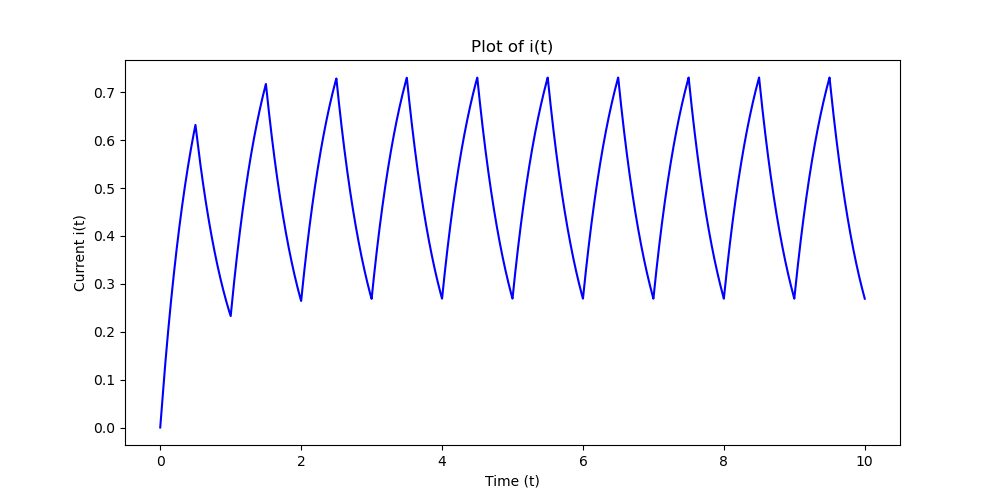
\includegraphics[width=0.8\linewidth]{figs/complete-fourier.png}
    \caption{Circuit Response using Fourier Series}
    \label{fig:enter-label}
\end{figure}